% !TeX TS-program = xelatex

% Load the required package using class
\documentclass[tikz,class=sagej]{standalone}


	% Additional packages
	\usepackage[]{pgfplots}                            % loads all the pgf packages
	\usepackage[]{contour}                           % for outlining text
	\usepackage{tikz-3dplot,comment,graphicx,bchart}
	\usepackage{mdframed,  tcolorbox,tkz-euclide}
	\usepackage{newtxtext}
	\usepackage[cmintegrals,cmbraces,varbb,nosymbolsc]{newtxmath}
	\usepackage{xfrac}

	\usetikzlibrary{spy,fit,matrix,shapes.callouts,calc,trees,positioning,arrows,chains,shapes.geometric,shapes.multipart,arrows.meta,  decorations.pathreplacing,decorations.text,decorations.pathmorphing,decorations.markings,shapes,matrix,shapes.symbols,patterns,datavisualization,datavisualization.formats.functions,angles,backgrounds}
	
	\usepgfplotslibrary{fillbetween,statistics}
	
	% Settings
	\pgfplotsset{compat=newest}

	% Math macros
	\newcommand{\fett}[1]{\mbox{\boldmath$#1$}} % only a help for smaller commands
	\renewcommand*{\vec}[1]{\lowercase{\fett{\sf#1}}} % vectors
	\newcommand{\mat}[1]{\uppercase{\fett{\sf#1}}} % matrices
	\newcommand{\tena}[1]{\lowercase{\fett{#1}}} % tensors 1. order
	\newcommand{\tenb}[1]{\uppercase{\fett{#1}}} % tensors 2. order
	\newcommand{\tend}[1]{{\uppercase{\fett{\mathcal#1}}}} % tensors 4. Stufe
	\newcommand{\dyad}{\otimes} % dyadic product
	\newcommand{\skp}{\fett{\cdot\,}} % scalar product
	\newcommand{\dskp}{\fett{:\,}} % double scalar product
	\newcommand{\equimust}{\stackrel{\mathrm{!}}{=}}


\pgfplotsset{
   compat=newest,
   xlabel near ticks,
   ylabel near ticks
}
 
 
 \usepgfplotslibrary{patchplots,colorbrewer}

\begin{document}

\begin{tikzpicture}
	\begin{scope}[spy using outlines={rectangle, black, connect spies, ultra thick}]
		\node at (0,0) {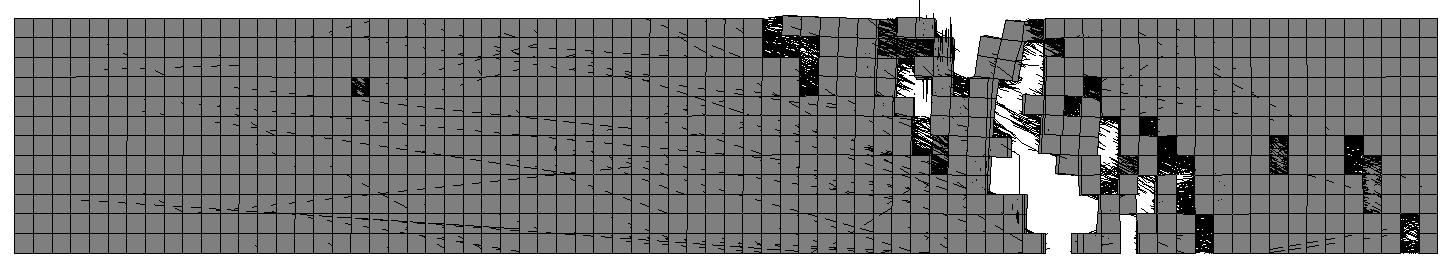
\includegraphics[scale=0.5]{fe_mesh.pdf}};
		\spy [size=5cm,magnification=2] on ($(2.5cm,0cm)$) in node at ($(-2,4cm)$);
		
	
	\end{scope}
%		\draw [line width=4pt,-{Latex[width'=0pt .5, length=25pt]}] (-12,9) -- +(-4,-2.7) node[below,pos=1] {\Huge \textbf{Warp}};	
%		\draw [line width=4pt,-{Latex[width'=0pt .5, length=25pt]}] (-13.5,7) -- +(+4,-3.3) node[below,pos=1] {\Huge \textbf{Weft}};	
\end{tikzpicture}



\end{document}
